%######################################################################################################################
% Title:        Thermal Model Order Reduction and Simulation (TherMOS)
% Topic:        Theory guide: model order reduction options
% File:         TherMOS_MOR_Theory.tex
% Date:         09.11.2026
% Author:       Dr. Pascal A. Schirmer
% Version:      V.1.0
% Copyright:    Pascal Schirmer
% Build:        latexmk -pdf TherMOS_MOR_Theory.tex   (or pdflatex twice)
%######################################################################################################################
\documentclass[11pt,a4paper]{article}

% ==============================================================================
% Packages
% ==============================================================================
\usepackage[T1]{fontenc}
\usepackage[utf8]{inputenc}
\usepackage{lmodern}
\usepackage[british]{babel}
\usepackage[margin=2.3cm]{geometry}
\usepackage{microtype}
\usepackage{amsmath,amssymb,mathtools,bm}
\usepackage{siunitx}
\usepackage{booktabs,tabularx,longtable,multirow}
\usepackage{enumitem}
\usepackage{xcolor}
\usepackage{tikz}
\usepackage[european,RPvoltages]{circuitikz}
\usepackage{pgfplots}
\usepackage[most]{tcolorbox}
\usepackage[hidelinks]{hyperref}
\usepackage[nameinlink,capitalise]{cleveref}

\pgfplotsset{compat=1.17}
\usepgfplotslibrary{groupplots}
\usetikzlibrary{arrows.meta,positioning,shapes.geometric,fit,calc}
\sisetup{per-mode=symbol,detect-all}
\setlist{nosep,leftmargin=*}
\setlength{\parindent}{0pt}
\setlength{\parskip}{0.55em}

% ==============================================================================
% Colours (business-research palette)
% ==============================================================================
\definecolor{cBlue}{HTML}{1F4E79}
\definecolor{cLight}{HTML}{DCE6F1}
\definecolor{cOrange}{HTML}{C55A11}
\definecolor{cGreen}{HTML}{548235}
\definecolor{cGrey}{HTML}{595959}
\definecolor{cRed}{HTML}{A50021}

\newtcolorbox{keybox}[1][Key point]{colback=cLight,colframe=cBlue,fonttitle=\bfseries,title=#1,arc=1mm,
  boxrule=0.6pt,left=2mm,right=2mm,top=1mm,bottom=1mm}
\newtcolorbox{examplebox}[1][Worked example]{colback=white,colframe=cOrange,fonttitle=\bfseries,title=#1,arc=1mm,
  boxrule=0.6pt,left=2mm,right=2mm,top=1mm,bottom=1mm}
\newtcolorbox{cfgbox}{colback=white,colframe=cGrey,fonttitle=\bfseries,title=Configuration in TherMOS,arc=1mm,
  boxrule=0.4pt,left=2mm,right=2mm,top=1mm,bottom=1mm,fontupper=\small}

% ==============================================================================
% Notation
% ==============================================================================
\newcommand{\Rth}{R_{\mathrm{th}}}
\newcommand{\Cth}{C_{\mathrm{th}}}
\newcommand{\Zth}{Z_{\mathrm{th}}}
\newcommand{\Tref}{T_{\mathrm{ref}}}
\newcommand{\T}{^{\mathsf T}}
\newcommand{\mat}[1]{\bm{#1}}
\newcommand{\cfg}[1]{\texttt{#1}}
\newcommand{\R}{\mathbb{R}}

\title{\textbf{TherMOS -- Thermal Model Order Reduction}\\[0.3em]
  \large Theory guide to the model order reduction options of the toolkit}
\author{Dr.\ Pascal A.\ Schirmer}
\date{Version 1.0, 9 November 2026}

\begin{document}
\maketitle

\begin{abstract}
\noindent
A detailed thermal model of a power electronic component -- a finite element (FE) or finite volume (FV) model with
thousands of nodes -- is accurate but far too slow for mission-profile simulations, lifetime estimation, design
optimisation or a temperature observer in a controller. Model order reduction (MOR) replaces it by a model with a few
states that reproduces the temperatures of interest. TherMOS offers eight reduced model families in its operating
modes (RC, SS, SF, PO, PS, ML, DL, PI) and two more in the board designer of the graphical user interface. They differ
in what they need (material data, measured profiles, single-source experiments), what they return (one temperature,
several junctions, the full field) and how safely they extrapolate. This guide derives every option from one common
full-order model, states every equation with its symbols and units, illustrates the key ideas with worked examples
computed with the toolkit, and ends with a selection guide.
\end{abstract}

\tableofcontents
\newpage

%######################################################################################################################
\section{How to read this guide}
%######################################################################################################################
\Cref{sec:fom} defines the full-order model that every reduced model approximates and shows its modal form. This form
is the key to the whole guide: it explains why a thermal system can be reduced at all and why Foster networks,
state-space models and POD models are three views of the same thing. \Cref{sec:lumped,sec:ss,sec:sf} treat the
\emph{lumped} models that reproduce a few temperatures (RC, SS, SF modes). \Cref{sec:pod,sec:ps,sec:board} treat the
\emph{field} models that reproduce the whole temperature field (PO and PS modes, board designer).
\Cref{sec:data,sec:pinn} treat the \emph{data-driven} and \emph{hybrid} models (ML, DL, PI modes).
\Cref{sec:select} compares all options and gives a selection guide; \cref{sec:metrics} defines the error metrics.
Every section ends with a box that names the configuration parameters (sheet \cfg{Mdl} of the configuration workbook,
GUI view \emph{Parameters}).

\begin{figure}[h]
\centering
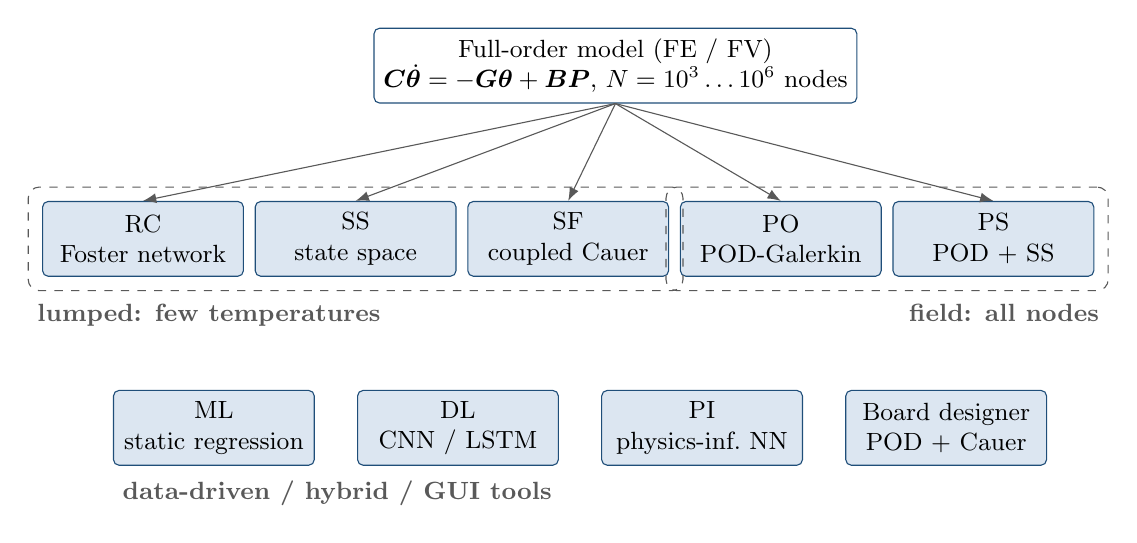
\begin{tikzpicture}[
  box/.style={draw=cBlue,fill=cLight,rounded corners=2pt,minimum width=2.55cm,minimum height=0.95cm,align=center,
              font=\small},
  grp/.style={draw=cGrey,dashed,rounded corners=4pt,inner sep=5pt},
  lab/.style={font=\small\bfseries,text=cGrey}]
  \node[box,fill=white,minimum width=5.5cm] (fom) at (0,2.2) {Full-order model (FE / FV)\\
        $\mat C\dot{\bm\theta}=-\mat G\bm\theta+\mat B\bm P$, $N=10^3\dots10^6$ nodes};
  \node[box] (rc) at (-6.0,0) {RC\\Foster network};
  \node[box] (ss) at (-3.3,0) {SS\\state space};
  \node[box] (sf) at (-0.6,0) {SF\\coupled Cauer};
  \node[box] (po) at (2.1,0) {PO\\POD-Galerkin};
  \node[box] (ps) at (4.8,0) {PS\\POD + SS};
  \node[box] (ml) at (-5.1,-2.4) {ML\\static regression};
  \node[box] (dl) at (-2.0,-2.4) {DL\\CNN / LSTM};
  \node[box] (pi) at (1.1,-2.4) {PI\\physics-inf.\ NN};
  \node[box] (bd) at (4.2,-2.4) {Board designer\\POD + Cauer};
  \node[grp,fit=(rc)(ss)(sf)] (g1) {};
  \node[grp,fit=(po)(ps)] (g2) {};
  \node[lab,below=1pt of g1.south west,anchor=north west] {lumped: few temperatures};
  \node[lab,below=1pt of g2.south east,anchor=north east] {field: all nodes};
  \foreach \n in {rc,ss,sf,po,ps} \draw[-{Latex},cGrey] (fom.south) -- (\n.north);
  \node[lab,below=2pt of ml.south west,anchor=north west] {data-driven / hybrid / GUI tools};
\end{tikzpicture}
\caption{Reduced model families of TherMOS. The lumped and field models approximate the full-order model directly
(by fitting its responses or by projecting its equations). The data-driven models learn the input--output map from
profiles; the PINN adds the physics of a lumped network to the training. The board designer builds its own FV model
and reduces it with POD and a coupled Cauer network.}
\label{fig:families}
\end{figure}

%######################################################################################################################
\section{The full-order model}\label{sec:fom}
%######################################################################################################################
\subsection{Heat equation}
The temperature $T(\bm x,t)$ in a solid with volumetric heat source $Q$ follows the heat equation
\begin{equation}
  \rho c\,\frac{\partial T}{\partial t} = \nabla\cdot\left(k\,\nabla T\right) - h_v\,(T-T_a) + Q(\bm x,t),
  \label{eq:heat}
\end{equation}
with convection $-k\,\partial T/\partial n = h\,(T-\Tref)$ or a fixed temperature on parts of the boundary and an
adiabatic rest. The distributed sink $h_v$ is used for thin boards whose cooling through the bottom side is smeared
over the area (board designer, \cref{sec:board}).

\begin{table}[h]\centering\small
\caption{Symbols of the full-order model.}
\begin{tabularx}{\linewidth}{@{}llX@{}}\toprule
Symbol & Unit & Meaning (typical value) \\\midrule
$T,\ T_a,\ \Tref$ & \si{\celsius} & temperature; ambient; reference temperature (coolant, heat sink, ambient) \\
$\theta = T-\Tref$ & \si{\kelvin} & temperature rise over the reference; all linear models work with $\theta$ \\
$\rho c$ & \si{\joule\per\cubic\metre\per\kelvin} & volumetric heat capacity (Cu \num{3.4e6}, Si \num{1.6e6}, FR4 \num{1.9e6}) \\
$k$ & \si{\watt\per\metre\per\kelvin} & thermal conductivity (Cu 390, Si 150, Al$_2$O$_3$ 25, FR4 0.3 through-plane) \\
$h,\ h_v$ & \si{\watt\per\square\metre\per\kelvin}, \si{\watt\per\cubic\metre\per\kelvin} & surface heat
  transfer coefficient (air 5--50, liquid cold plate 1000--20000); distributed sink per volume \\
$Q$ & \si{\watt\per\cubic\metre} & volumetric heat generation (losses of a chip divided by its volume) \\
$N$ & -- & number of nodes of the discretised model ($10^3$--$10^6$) \\
$S$ & -- & number of loss sources (chips, windings) \\
$\bm\theta\in\R^N$ & \si{\kelvin} & node temperature rises \\
$\bm P\in\R^S$ & \si{\watt} & losses of the sources \\
$\mat C\in\R^{N\times N}$ & \si{\joule\per\kelvin} & capacitance matrix: diagonal (FV) or consistent mass matrix (FE), positive definite \\
$\mat G\in\R^{N\times N}$ & \si{\watt\per\kelvin} & conductance matrix: symmetric, positive definite if any heat leaves the body \\
$\mat B\in\R^{N\times S}$ & -- & input matrix: share of loss $j$ that enters node $i$ (columns sum to 1) \\
$\mat L\in\R^{p\times N}$ & -- & output matrix: selects (or averages) the $p$ temperatures of interest \\\bottomrule
\end{tabularx}
\label{tab:fomsym}
\end{table}

\subsection{Semi-discrete form}
An FE or FV discretisation of \eqref{eq:heat} gives a linear system of $N$ ordinary differential equations
\begin{equation}
  \mat C\,\dot{\bm\theta}(t) = -\mat G\,\bm\theta(t) + \mat B\,\bm P(t), \qquad \bm y(t) = \mat L\,\bm\theta(t).
  \label{eq:fom}
\end{equation}
For the FV model of the board designer (\texttt{calcBoardMat}) every node $i$ owns the control volume $V_i$; the
entries are
\begin{equation}
  C_i = (\rho c)_i V_i,\qquad G_{ij} = -\frac{A_{ij}}{d/(2k_i)+d/(2k_j)}\ (i\neq j\ \text{neighbours}),\qquad
  G_{ii} = \sum_{j\neq i}|G_{ij}| + h_{v,i}V_i,
\end{equation}
with $A_{ij}$ the face between the volumes and $d$ the node distance. Three properties hold for every thermal model
and are used throughout the guide:
\begin{enumerate}
  \item \textbf{Passivity.} $\mat C$ and $\mat G$ are symmetric positive definite. The stored energy
        $\tfrac12\bm\theta\T\mat C\bm\theta$ can only fall without losses: the model is stable and does not oscillate.
  \item \textbf{Linearity.} With temperature-independent $\rho c$, $k$, $h$ the response to several sources is the
        sum of the responses to each source (superposition). Thermal impedances and resistance matrices rely on it.
  \item \textbf{Steady state.} For constant losses $\bm\theta_\infty = \mat G^{-1}\mat B\bm P$. The thermal resistance
        matrix $\Rth = \mat L\mat G^{-1}\mat B$ (\si{\kelvin\per\watt}) collects self-heating (diagonal) and
        cross-heating (off-diagonal).
\end{enumerate}

\subsection{Modal form: why thermal models can be reduced}\label{sec:modal}
The generalised eigenvalue problem
\begin{equation}
  \mat G\,\bm v_k = \lambda_k\,\mat C\,\bm v_k,\qquad \mat V\T\mat C\mat V = \mat I,\quad \mat V\T\mat G\mat V =
  \bm\Lambda = \mathrm{diag}(\lambda_1,\dots,\lambda_N),\quad 0<\lambda_1\le\lambda_2\le\dots
  \label{eq:gevp}
\end{equation}
has $N$ real positive eigenvalues $\lambda_k$ (\si{\per\second}) because $\mat C$ and $\mat G$ are symmetric
positive definite. With $\bm\theta = \mat V\bm z$, \eqref{eq:fom} falls apart into $N$ independent first-order
systems $\dot z_k = -\lambda_k z_k + \bm v_k\T\mat B\bm P$. The response of output $i$ to a \SI{1}{\watt} step in
source $j$ -- the \emph{thermal impedance} -- is therefore a sum of exponentials:
\begin{equation}
  \boxed{\;Z_{ij}(t) = \sum_{k=1}^{N} R_{ijk}\left(1-e^{-t/\tau_k}\right),\qquad
  \tau_k = \frac{1}{\lambda_k},\qquad R_{ijk} = \frac{(\mat L\bm v_k)_i\,(\bm v_k\T\mat B)_j}{\lambda_k}\;}
  \label{eq:modalZ}
\end{equation}
This is a Foster network with $N$ RC pairs. Its time constants $\tau_k$ are the same for all inputs and outputs; only
the weights $R_{ijk}$ change. For self-heating with collocated input and output ($\mat L = \mat B\T$) every
$R_{iik} = (\bm v_k\T\bm b_i)^2/\lambda_k$ is positive, for cross-heating ($i\ne j$) single terms can be negative.

\begin{keybox}[Why a few states are enough]
Two facts make the reduction work. (1) The time constants are spread over many decades (chip
\SIrange{1}{10}{\milli\second}, substrate \SIrange{0.1}{1}{\second}, heat sink \SIrange{10}{1000}{\second}); a
sampled model with $T_s=\SI{1}{\second}$ cannot see modes with $\tau_k\ll T_s$ -- they are quasi-static. (2) Most
modes are hardly excited by the chip losses or hardly seen at the sensors: their weights $R_{ijk}$ are tiny. Typically
3--8 modes carry more than \SI{99.9}{\percent} of the response. Every reduced model in this guide is a way to find
these few modes -- by fitting (RC, SS, SF, PS), by projection (PO) or by learning (ML, DL, PI).
\end{keybox}

\begin{examplebox}[Worked example 1: two-node chain]
A chip ($C_1=\SI{2}{\joule\per\kelvin}$) sits on a heat sink ($C_2=\SI{40}{\joule\per\kelvin}$) with
$R_{12}=\SI{0.5}{\kelvin\per\watt}$ between them and $R_{2a}=\SI{1.0}{\kelvin\per\watt}$ to the coolant:
\[
  \mat C = \begin{bmatrix}2&0\\0&40\end{bmatrix},\qquad
  \mat G = \begin{bmatrix}2&-2\\-2&3\end{bmatrix}\si{\watt\per\kelvin},\qquad \mat B = \mat L\T =
  \begin{bmatrix}1\\0\end{bmatrix}.
\]
\eqref{eq:gevp} gives $\lambda_1=\SI{0.0238}{\per\second}$, $\lambda_2=\SI{1.051}{\per\second}$, i.e.
$\tau_1=\SI{42.0}{\second}$ (heat sink) and $\tau_2=\SI{0.951}{\second}$ (chip). The Foster weights of the chip are
$R_1=\SI{1.048}{\kelvin\per\watt}$ and $R_2=\SI{0.452}{\kelvin\per\watt}$; their sum is the steady-state resistance
$[\mat G^{-1}]_{11}=R_{12}+R_{2a}=\SI{1.5}{\kelvin\per\watt}$. Note that neither Foster pair equals a physical part:
$\tau_2=\SI{0.951}{\second}$ is not $R_{12}C_1=\SI{1}{\second}$, and $R_1\neq R_{2a}$. \Cref{fig:zth} shows the curve.
\end{examplebox}

\begin{figure}[h]\centering
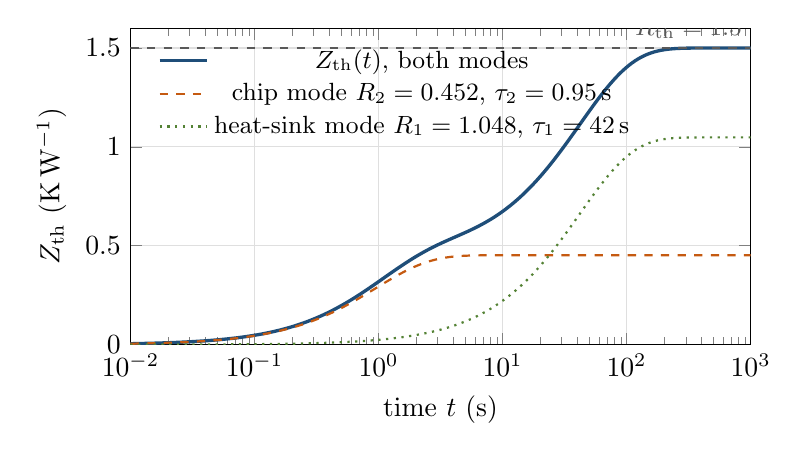
\begin{tikzpicture}
\begin{axis}[width=0.78\linewidth,height=5.6cm,xmode=log,xmin=1e-2,xmax=1e3,ymin=0,ymax=1.6,
  xlabel={time $t$ (\si{\second})},ylabel={$\Zth$ (\si{\kelvin\per\watt})},grid=major,grid style={gray!25},
  legend pos=north west,legend style={font=\small,draw=none,fill=none},samples=200,domain=1e-2:1e3]
  \addplot[cBlue,very thick] {1.04807*(1-exp(-x/42.0487))+0.451928*(1-exp(-x/0.951277))};
  \addlegendentry{$\Zth(t)$, both modes}
  \addplot[cOrange,thick,dashed] {0.451928*(1-exp(-x/0.951277))};
  \addlegendentry{chip mode $R_2=0.452$, $\tau_2=0.95\,$s}
  \addplot[cGreen,thick,dotted] {1.04807*(1-exp(-x/42.0487))};
  \addlegendentry{heat-sink mode $R_1=1.048$, $\tau_1=42\,$s}
  \draw[cGrey,dashed] (axis cs:1e-2,1.5) -- (axis cs:1e3,1.5) node[pos=0.9,above,font=\small] {$\Rth=1.5$};
\end{axis}
\end{tikzpicture}
\caption{Thermal impedance of worked example 1 on a logarithmic time axis. Each Foster term is an S-curve centred on
its time constant; the chip mode settles after about $3\tau_2\approx\SI{3}{\second}$, the heat-sink mode after about
$3\tau_1\approx\SI{2}{\minute}$. After about \SI{200}{\second} the curve reaches $\Rth=\SI{1.5}{\kelvin\per\watt}$:
\SI{10}{\watt} of losses heat the chip by \SI{15}{\kelvin}.}
\label{fig:zth}
\end{figure}

%######################################################################################################################
\section{Thermal networks: Foster and Cauer (RC mode)}\label{sec:lumped}
%######################################################################################################################
\subsection{Foster network}
The RC mode reproduces one temperature (the first output channel) from one loss with a Foster network of $K$ RC pairs
in series, i.e.\ \eqref{eq:modalZ} truncated to the $K$ dominant modes:
\begin{equation}
  \Zth(t) = \sum_{k=1}^{K} R_k\left(1-e^{-t/\tau_k}\right),\qquad \tau_k = R_kC_k,\qquad
  \Rth = \sum_k R_k .
  \label{eq:foster}
\end{equation}
For an arbitrary loss profile the response is the convolution of the impulse response $\mathrm d\Zth/\mathrm dt$ with
$P(t)$. TherMOS evaluates it recursively for every pair (\texttt{rcSim}, trapezoidal/Tustin rule, exact for losses
that are linear between the samples):
\begin{equation}
  \theta_k(n) = \frac{2\tau_k - T_s}{2\tau_k+T_s}\,\theta_k(n-1) + \frac{R_kT_s}{2\tau_k+T_s}\bigl(P(n)+P(n-1)\bigr),
  \qquad T(n) = \Tref(n) + \sum_{k=1}^{K}\theta_k(n).
  \label{eq:tustin}
\end{equation}

\begin{figure}[h]\centering
\begin{circuitikz}[scale=0.82,transform shape,font=\small]
  % Foster
  \draw (0,0) node[left]{$T_j$} to[short,o-] (0.5,0);
  \draw (0.5,0) -- (0.5,0.8) to[R,l=$R_1$] (2.5,0.8) -- (2.5,0);
  \draw (0.5,0) -- (0.5,-0.8) to[C,l_=$C_1$] (2.5,-0.8) -- (2.5,0);
  \draw (2.5,0) -- (3,0);
  \draw (3,0) -- (3,0.8) to[R,l=$R_2$] (5,0.8) -- (5,0);
  \draw (3,0) -- (3,-0.8) to[C,l_=$C_2$] (5,-0.8) -- (5,0);
  \draw (5,0) -- (5.5,0) node[right]{$\cdots$};
  \draw (6.3,0) -- (6.8,0);
  \draw (6.8,0) -- (6.8,0.8) to[R,l=$R_K$] (8.8,0.8) -- (8.8,0);
  \draw (6.8,0) -- (6.8,-0.8) to[C,l_=$C_K$] (8.8,-0.8) -- (8.8,0);
  \draw (8.8,0) to[short,-o] (9.3,0) node[right]{$\Tref$};
  \node[font=\small\bfseries] at (4.6,1.7) {Foster: $Z(s)=\sum_k \dfrac{R_k}{1+s\tau_k}$};
  % Cauer
  \begin{scope}[yshift=-3.6cm]
  \draw (0,0) node[left]{$T_j$} to[short,o-] (0.5,0) to[R,l=$R'_1$] (2.5,0) to[R,l=$R'_2$] (4.5,0)
        -- (5,0) node[right]{$\cdots$};
  \draw (6.1,0) -- (6.5,0);
  \draw (6.5,0) to[R,l=$R'_K$] (8.5,0) to[short,-o] (9.3,0) node[right]{$\Tref$};
  \draw (0.5,0) to[C,l=$C'_1$,*-] (0.5,-1.4) node[ground]{};
  \draw (2.5,0) to[C,l=$C'_2$,*-] (2.5,-1.4) node[ground]{};
  \draw (4.5,0) to[C,l=$C'_3$,*-] (4.5,-1.4) node[ground]{};
  \draw (6.5,0) to[C,l=$C'_K$,*-] (6.5,-1.4) node[ground]{};
  \node[font=\small\bfseries] at (4.6,1.0) {Cauer: ladder, every node a physical temperature};
  \end{scope}
\end{circuitikz}
\caption{Foster (top) and Cauer (bottom) form of a heat path from the junction $T_j$ to the reference $\Tref$. Both
have the same impedance $Z(s)$ when the Cauer parameters are computed from the Foster ones. The capacitances of the
Cauer ladder are grounded (connected to thermal ground, \SI{0}{\kelvin} rise), those of the Foster network sit
across the resistances -- they have no physical meaning.}
\label{fig:fostercauer}
\end{figure}

\subsection{Fit of the Foster parameters}
TherMOS fits the $2K$ parameters by an \emph{output-error} least-squares fit: the network \eqref{eq:tustin} is
simulated with the measured losses of all training profiles and compared with the measured temperature rise
$\Delta T(n)=T(n)-T(0)$:
\begin{equation}
  \min_{\ln R_k,\ \ln\tau_k}\ \sum_{\text{profiles}}\ \sum_{n}\bigl(\theta_{\mathrm{sim}}(n) - \Delta
  T_{\mathrm{meas}}(n)\bigr)^2 .
\end{equation}
Logarithmic parameters keep $R_k$ and $\tau_k$ positive and give the time constants that span several decades
comparable step sizes; the start values of $\tau_k$ are spread logarithmically between $T_s$ and the profile length.
Unlike the classical fit of \eqref{eq:foster} to $\Delta T/P$ (MATLAB version, \cfg{legacy = 1}) the output-error fit
works for any loss profile, not only for a constant step.

\textbf{What the fit can and cannot identify.} $\Rth$ is always well determined. The split into pairs is not unique:
pairs with $\tau_k$ within a factor of about 3 are hard to separate, and time constants that the profile does not
excite (shorter than $T_s$, longer than the profile) cannot be found. Pulse profiles excite the fast modes better than
a single step.

\subsection{Cauer network and structure function}
A Cauer ladder (\cref{fig:fostercauer}, bottom) has the same impedance as a Foster network when its parameters follow
from the continued-fraction expansion of the Foster admittance (\texttt{foster2cauer}):
\begin{equation}
  Z(s) = \sum_{k=1}^{K}\frac{R_k}{1+s\tau_k} = \cfrac{1}{sC'_1 + \cfrac{1}{R'_1 + \cfrac{1}{sC'_2 +
  \cfrac{1}{R'_2+\dotsb}}}}
\end{equation}
For worked example 1 the expansion returns exactly the physical ladder $R'=(0.5,\,1.0)\,\si{\kelvin\per\watt}$,
$C'=(2,\,40)\,\si{\joule\per\kelvin}$: a Cauer ladder is unique and its nodes can be physical temperatures if the heat
path really is one-dimensional. Plotting the cumulative capacitance $\sum_{k\le m}C'_k$ over the cumulative resistance
$\sum_{k\le m}R'_k$ gives the \emph{cumulative structure function} (JEDEC JESD51-14 \cite{jesd51}); flat parts are
layers with a high resistance and little mass (solder, thermal interface), steep parts are heavy layers with a low
resistance (baseplate, heat sink). The GUI page \emph{Theory \& Tools › Thermal networks} converts Foster to Cauer and
draws the structure function.

\begin{keybox}[Interpretation]
Use a Foster network to \emph{simulate} a heat path (simple, exact for the fitted path). Convert it to Cauer to
\emph{connect} paths (e.g.\ a module network to a heat-sink network) or to \emph{interpret} it (structure function):
Foster networks cannot be connected in series because their inner nodes are not temperatures.
\end{keybox}

\begin{cfgbox}
\cfg{Mdl › rc › K}: number of RC pairs $K$ (3--5 for chip, solder, substrate, heat sink).
\cfg{Mdl › gen › opt = 1}: order search $K=1\dots$\cfg{Kmax} on the validation data.
\cfg{Mdl › rc › bc}: parameter bound of the MATLAB fit (\cfg{legacy = 1} only).
Only the first input/output pair is used; for several coupled outputs use the SS or SF mode.
\end{cfgbox}

%######################################################################################################################
\section{State-space identification (SS mode)}\label{sec:ss}
%######################################################################################################################
\subsection{Model}
The SS mode identifies one multiple-input multiple-output (MIMO) model for all $m$ losses and $p$ temperatures:
\begin{equation}
  \bm x(n+1) = \mat A\,\bm x(n) + \mat B_d\,\bm u(n),\qquad \bm y(n) = \mat C_o\,\bm x(n),
  \label{eq:ss}
\end{equation}
with $\bm u=\bm P$ (\si{\watt}), $\bm y=\bm\theta$ (\si{\kelvin}), $n_x$ states $\bm x$ without physical meaning and
no direct feedthrough. A continuous model $\dot{\bm x}=\mat A_c\bm x+\mat B_c\bm u$ sampled with zero-order hold
gives
\begin{equation}
  \mat A = e^{\mat A_cT_s},\qquad \mat B_d = \mat A_c^{-1}\bigl(\mat A-\mat I\bigr)\mat B_c,\qquad
  z_k = e^{-T_s/\tau_k}\ \Leftrightarrow\ \tau_k = -\frac{T_s}{\ln z_k}.
  \label{eq:zoh}
\end{equation}
For a thermal system the discrete poles $z_k=\mathrm{eig}(\mat A)$ are real with $0<z_k<1$: $z_k\to1$ is a slow
mode, $z_k\to0$ a fast one. Complex or negative poles indicate an over-fitted order. Compared with the RC mode the
SS model shares the time constants between all channels (\eqref{eq:modalZ}) and includes cross-heating.

\subsection{Subspace identification (N4SID/MOESP)}
TherMOS uses the past-output MOESP algorithm \cite{verhaegen,vanoverschee} (\texttt{fitN4sid}, the counterpart of
MATLAB \texttt{n4sid}). With $s$ block rows (horizon) the inputs are arranged in a block Hankel matrix
\begin{equation}
  \mat U = \begin{bmatrix} \bm u(0) & \bm u(1) & \cdots & \bm u(J-1)\\ \bm u(1) & \bm u(2) & \cdots & \bm u(J)\\
  \vdots & & & \vdots\\ \bm u(2s-1) & \cdots & & \bm u(2s+J-2)\end{bmatrix}
  = \begin{bmatrix}\mat U_p\\ \mat U_f\end{bmatrix},
\end{equation}
split into past ($p$) and future ($f$) halves; $\mat Y_p$, $\mat Y_f$ likewise. Repeated substitution of
\eqref{eq:ss} gives the data equation
\begin{equation}
  \mat Y_f = \bm\Gamma_s\,\mat X_f + \mat H_s\,\mat U_f,\qquad
  \bm\Gamma_s = \begin{bmatrix}\mat C_o\\ \mat C_o\mat A\\ \vdots\\ \mat C_o\mat A^{s-1}\end{bmatrix},\qquad
  \mat H_s = \begin{bmatrix}\mat 0 & & \\ \mat C_o\mat B_d & \mat 0 & \\ \mat C_o\mat A\mat B_d & \mat C_o\mat B_d &
  \ddots\end{bmatrix}
\end{equation}
with the extended observability matrix $\bm\Gamma_s$ and the Toeplitz matrix $\mat H_s$ of the Markov parameters.
The algorithm
\begin{enumerate}
  \item computes the LQ decomposition of $[\mat U_f;\ \mat W_p;\ \mat Y_f]$ with $\mat W_p=[\mat U_p;\ \mat Y_p]$; the
        block that maps $\mat W_p$ to $\mat Y_f$ after removing $\mat U_f$ equals $\bm\Gamma_s\mat X_f$ seen through
        the past data;
  \item takes its singular value decomposition $\mat U\bm\Sigma\mat V\T$. The number of significant singular values is
        the \textbf{model order}: the largest gap on a log scale is chosen when a list of orders is given;
  \item sets $\bm\Gamma_s=\mat U_1\bm\Sigma_1^{1/2}$ and reads $\mat C_o$ from its first block row and $\mat A$ from
        the shift structure $\underline{\bm\Gamma}_s\mat A = \overline{\bm\Gamma}_s$ (all block rows but the last
        resp.\ the first) by least squares;
  \item finds $\mat B_d$ (and the initial states $\bm x_0$ of the profiles) by linear least squares on the simulated
        output.
\end{enumerate}
Several profiles are stacked column-wise, so the model is fitted to all experiments at once. If no horizon is given
the horizon with the smallest simulation error is chosen from a set of candidates.

\subsection{Output-error refinement}
The subspace estimate minimises an algebraic criterion. Option \cfg{dis = 2} refines it with the prediction-error
method in output-error form \cite{ljung} (\texttt{fitPem}, MATLAB \texttt{ssest} without a noise model):
\begin{equation}
  \min_{\mat A,\mat B_d,\mat C_o,\bm x_0}\ \sum_{e}\sum_{n}\bigl\lVert \bm y_e(n) - \hat{\bm y}_e(n)\bigr\rVert^2 ,
\end{equation}
where $\hat{\bm y}_e$ is the free simulation of experiment $e$. It has $n_x^2+n_xm+pn_x$ parameters. With
\cfg{sta = 2} unstable poles are mirrored into the unit circle ($z\to1/z^*$) and $\mat B_d$, $\bm x_0$ are refitted.

\begin{keybox}[Choosing the order]
$n_x$ is about the number of time constants that the data excite and that the sampling resolves. Too small an order
merges time constants (the fast rise or the slow tail is missed); too large an order fits noise and produces complex
or unstable poles. Start with the number of outputs $+1$ and check the singular value plot of the GUI (\emph{Theory}
view of the SS mode): a clear gap after $\sigma_{n}$ supports order $n$.
\end{keybox}

\begin{cfgbox}
\cfg{Mdl › ss › K}: order $n_x$. \cfg{Mdl › ss › dis}: 1 subspace only, 2 subspace + output-error fit.
\cfg{Mdl › ss › init}: 1 zero initial state, 2 estimated. \cfg{Mdl › ss › sta}: 2 enforces stability.
\cfg{Mdl › ss › sol}: 1 free simulation from the initial state, 2 as MATLAB \texttt{compare}.
\end{cfgbox}

%######################################################################################################################
\section{Coupled heat sources (SF mode)}\label{sec:sf}
%######################################################################################################################
Power modules carry several chips on one substrate; each chip heats its neighbours. The SF mode builds a nodal
network of $M$ coupled sources with $K$ stages each:
\begin{equation}
  \mat C\,\dot{\bm\theta} = \mat E\,\bm P(t) - \mat G\,\bm\theta,\qquad
  \bm\theta_j = [\bm\theta]_{\text{junctions}},\qquad \Rth = \bigl[\mat G^{-1}\bigr]_{jj}.
  \label{eq:sf}
\end{equation}
$\mat C$ is diagonal (one capacitance per node), $\mat E$ puts the loss of chip $i$ into its junction node, and
$\mat G$ is assembled from the ladder and coupling resistances:
\begin{equation}
  \mat G = \sum_{i,k}\frac{1}{R'_{ik}}\,(\bm e_{ik}-\bm e_{i,k+1})(\bm e_{ik}-\bm e_{i,k+1})\T
         + \sum_{i<j,\,k}\frac{1}{R_{ij,k}}\,(\bm e_{ik}-\bm e_{jk})(\bm e_{ik}-\bm e_{jk})\T ,
\end{equation}
where $\bm e_{ik}$ is the unit vector of stage $k$ of chip $i$ and the last stage connects to $\Tref$
($\bm e_{i,K+1}=\bm 0$).

\begin{table}[h]\centering\small
\caption{Symbols of the coupled network.}
\begin{tabularx}{\linewidth}{@{}llX@{}}\toprule
Symbol & Unit & Meaning \\\midrule
$M$, $K$ & -- & number of heat sources (chips); stages per chip (\cfg{Mdl › rc › K}) \\
$R'_{ik}$, $C'_{ik}$ & \si{\kelvin\per\watt}, \si{\joule\per\kelvin} & resistance and capacitance of stage $k$ of chip $i$ (stage 1 = junction) \\
$R_{ij,k}$ & \si{\kelvin\per\watt} & coupling resistance between stage $k$ of chips $i$ and $j$ (large = weak coupling) \\
$\Rth\in\R^{M\times M}$ & \si{\kelvin\per\watt} & steady-state resistance matrix; column $j$: rise of all junctions for \SI{1}{\watt} in chip $j$ \\
$b$ & -- & bound factor of the fit (\cfg{Mdl › sf › bnd}) \\\bottomrule
\end{tabularx}
\end{table}

\subsection{Method 2 (default): coupled Cauer network fitted to any profile}
All parameters are found by a bounded output-error fit (trust-region reflective):
\begin{equation}
  \min_{\bm p}\ \sum_n \bigl\lVert \bm T(n) - \hat{\bm T}(n;\bm p)\bigr\rVert^2,\qquad
  \bm p = \ln\bigl[R'_{ik},\ C'_{ik},\ 1/R_{ij,k}\bigr],\qquad \bm p_0 - \ln b \le \bm p \le \bm p_0 + \ln b .
\end{equation}
The log-parameters keep every $R$ and $C$ positive, so every candidate is passive and stable. The start values are
$R'_{ik}=R_{\mathrm{th},i}/K$ (from a least-squares fit of the last fifth of every profile), time constants spaced
logarithmically between $T_s/2$ and a third of the profile length, and couplings $1/R_{ij,k}=0.1/\overline{R}_{\mathrm{th}}$.
Long data are decimated to \cfg{Nmax} samples. The network is simulated exactly for losses held constant over a
sample (\texttt{sfNet}): with $\mat S=\mat C^{1/2}$ and $\mat S^{-1}\mat G\mat S^{-1}=\mat V\bm\Lambda\mat V\T$,
\begin{equation}
  z_k(n+1) = e^{-\lambda_kT_s}z_k(n) + \frac{1-e^{-\lambda_kT_s}}{\lambda_k}\,b_k(n),\qquad
  \bm b = \mat V\T\mat S^{-1}\mat E\bm P,\qquad \bm\theta = \mat S^{-1}\mat V\bm z .
\end{equation}

\subsection{Method 1 (MATLAB): nodal Foster model}
For every chip $k$ a Foster network is fitted to the self-heating curve of an experiment in which only chip $k$ is
heated; the steady-state matrix $R_{\mathrm{th},ik}=\Delta T_i(\infty)/P_k$ is symmetrised and inverted
($\mat G=\Rth^{-1}$). It needs one single-source experiment per chip. Its ODE time constants differ from the fitted
Foster pairs, so its dynamics are approximate. With fewer experiments than chips TherMOS falls back to method 2.

\begin{keybox}[Identifiability]
Superposition gives the junction rise $\theta_i = \sum_j R_{\mathrm{th},ij}P_j$ in steady state. If two chips always
carry the same loss (diagonal switches of a full bridge), the data only show the sum of their columns; the fitted
network predicts this operation well, but the individual entries of $\Rth$ are not unique. Add single-chip steps
to the training data to separate self- and cross-heating. Couplings that end at the lower bound are negligible.
\end{keybox}

\begin{cfgbox}
Setup \cfg{selSF}: 1 nodal Foster, 2 coupled Cauer network. \cfg{Mdl › rc › K}: stages per chip.
\cfg{Mdl › sf › bnd}: bound factor $b$. \cfg{Mdl › sf › Nmax}: maximum samples of the fit.
\end{cfgbox}

%######################################################################################################################
\section{Proper orthogonal decomposition and Galerkin projection (PO mode)}\label{sec:pod}
%######################################################################################################################
The lumped models reproduce a few temperatures. The PO mode reproduces the \emph{whole field}, e.g.\ to find the
hottest point of a board whose position changes with the load \cite{thermos}.

\subsection{Proper orthogonal decomposition (POD)}
The temperature field is approximated by $K$ spatial modes $\phi_i(\bm x)$ with time coefficients $a_i(t)$:
\begin{equation}
  T(\bm x,t) \approx T_0(\bm x) + \sum_{i=1}^{K}\phi_i(\bm x)\,a_i(t),\qquad
  \bm T(t) \approx \bm T_0 + \bm\Phi\,\bm a(t),\quad \bm\Phi\in\R^{N\times K}.
  \label{eq:podexp}
\end{equation}
POD chooses the basis that represents the $N_t$ training snapshots $\bm\theta(t_1),\dots,\bm\theta(t_{N_t})$ (columns of
$\bm\Theta\in\R^{N\times N_t}$, mean-centred in the PO mode) with the smallest mean square error \cite{holmes}:
\begin{equation}
  \min_{\bm\Phi\T\bm\Phi=\mat I}\ \sum_{t}\bigl\lVert \bm\theta(t) - \bm\Phi\bm\Phi\T\bm\theta(t)\bigr\rVert^2
  = \sum_{i>K}\sigma_i^2,\qquad \bm\Theta = \mat U\bm\Sigma\mat W\T,\quad \bm\Phi = \mat U_{:,1..K}.
\end{equation}
The minimum is reached by the first $K$ left singular vectors (Eckart--Young theorem); the residual is the sum of the
discarded squared singular values $\sigma_i$. The \emph{captured energy}
\begin{equation}
  E_K = \frac{\sum_{i\le K}\sigma_i^2}{\sum_i\sigma_i^2}
\end{equation}
selects $K$ (\cfg{Mdl › pod › sel = 2}: smallest $K$ with $E_K\ge$ \cfg{Emax}). Mode 1 is the mean heating pattern,
the next modes describe how the sources heat differently and how the heat spreads.

\begin{keybox}[POD versus modal truncation]
The eigenvectors $\bm v_k$ of \eqref{eq:gevp} are also a reduction basis (\emph{modal truncation}: keep the slowest
$K$). They depend only on the system. POD modes depend on the training load: they are optimal for loads like the
training load but can miss a source that was never active in training. Train the POD on profiles in which every source
is active with different amplitudes (random levels are better than one synchronous step). The GUI page
\emph{Theory \& Tools › MOR \& POD} compares both bases on a 1D rod.
\end{keybox}

\subsection{Galerkin projection}
Inserting \eqref{eq:podexp} into the heat equation and requiring the residual to be orthogonal to every mode
(weak form, test functions $\phi_i$) gives $K$ ordinary differential equations
\begin{equation}
  \mat C_r\,\dot{\bm a} = -\mat G_r\,\bm a + \bm\alpha\circ\bm q(t),
  \label{eq:galerkin}
\end{equation}
\begin{equation}
  C_{r,ij} = \int_\Omega \rho c\,\phi_i\phi_j\,\mathrm d\Omega,\quad
  G_{r,ij} = \int_\Omega\bigl(k\,\partial_x\phi_i\partial_x\phi_j + k_y\,\partial_y\phi_i\partial_y\phi_j +
  h_v\,\phi_i\phi_j\bigr)\mathrm d\Omega,\quad
  q_i = \int_\Omega Q\,\phi_i\,\mathrm d\Omega .
\end{equation}
$\bm\alpha$ is a load correction ($\bm\alpha=\bm 1$ for the pure projection). For a discretised model the same
projection reads $\mat C_r=\bm\Phi\T\mat C\bm\Phi$, $\mat G_r=\bm\Phi\T\mat G\bm\Phi$, $\bm q=\bm\Phi\T\mat B\bm P$;
it keeps symmetry and positive definiteness, so the projected model is stable and passive. In the PO mode the modes
are given at scattered FE nodes; they are interpolated to a regular grid and the integrals are evaluated with
Gauss--Legendre quadrature ($\int f\,\mathrm d\Omega\approx\sum_q W_qf(\bm x_q)$, \texttt{calcPodQuad},
\texttt{calcPodProj}). The ODE is solved exactly with the matrix exponential for losses linear between samples,
starting from $\bm a(0)=\bm 0$ at the measured initial field $\bm T_0$.

\textbf{Assumptions.} Mean-centred modes vanish on fixed-temperature boundaries, so no boundary term appears.
Convective boundaries must be part of $\mat G_r$ ($h_v$ for boards): without the heat sink the projected model has no
path for the heat to leave, and the temperature rises without bound (\cref{tab:podex}).

\subsection{Calibration protocols}
FE data often do not contain every physical detail (contact resistances, the real cooling), and the interpolation and
quadrature add errors. Protocols 4--6 therefore correct the projected matrices with the training data. With the
modal coordinates $\bm a(t)=\bm\Phi\T(\bm T(t)-\bm T_0)$, their central-difference derivatives $\dot{\bm a}$ and the
projected loads $\bm q$, all problems are linear least squares (equation error, \texttt{optPodMat}):

\begin{table}[h]\centering\small
\caption{POD protocols (\cfg{Mdl › pod › protocol}).}\label{tab:protocols}
\begin{tabularx}{\linewidth}{@{}clX@{}}\toprule
No. & Reduced matrices & Use \\\midrule
1 & unweighted sum over the nodes & MATLAB behaviour only (\cfg{legacy = 1}) \\
2 & Gauss--Legendre projection (pure Galerkin) & physics only; extrapolates safely if the data contain all heat paths \\
3 & as 2 (legacy: relative element size) & physics only \\
4 & 2 + steady-state load correction $\min_{\bm\alpha}\lVert\mat G_r\bm a-\bm\alpha\circ\bm q\rVert^2$ & physics + one calibration vector \\
5 & $\min_{\mat C_r,\mat G_r}\lVert\bm q-\mat C_r\dot{\bm a}-\mat G_r\bm a\rVert^2$, then $\bm\alpha$ & data-calibrated (default), most accurate on FE or measured data \\
6 & as 5 $+\,\lambda\bigl(\lVert\mat C_r-\mat C_{r0}\rVert^2+\lVert\mat G_r-\mat G_{r0}\rVert^2\bigr)$, $\lambda=10^{-3}$ & regularised towards the projection; robust with little data \\\bottomrule
\end{tabularx}
\end{table}

Protocol 5 is underdetermined for modes with almost no energy and for pure step responses (the regressors
$\dot{\bm a}$ and $\bm a$ then span only the exponentials of the response and cannot separate $\mat C_r$ from
$\mat G_r$). TherMOS solves it per mode with a truncated SVD (singular values below $10^{-3}$ of the largest are
dropped) as the minimum-norm correction of the projected matrices, and keeps the projected matrices if the calibrated
model is singular or unstable.

\begin{examplebox}[Worked example 2: POD-Galerkin of a DBC board]
Board designer model of a 40\,mm $\times$ 30\,mm DBC (Al$_2$O$_3$ on a \SI{3}{\milli\metre} Cu baseplate,
$h=\SI{1000}{\watt\per\square\metre\per\kelvin}$, $T_a=\SI{25}{\celsius}$) with an IGBT (\SI{40}{\watt}) and a diode
(\SI{15}{\watt}) on a \SI{1}{\milli\metre} grid, $N=1271$ nodes. Training: \SI{600}{\second} of random loss levels;
test: pulse trains with periods of \SI{120}{\second} and \SI{200}{\second} (maximum rise \SI{50.5}{\kelvin}).
The snapshots are not centred here ($\theta=T-T_a$). \Cref{tab:podex} lists the result; \cref{fig:pod} shows the
singular values and the error.
\end{examplebox}

\begin{table}[h]\centering\small
\caption{Worked example 2: maximum absolute error on the test profile over the number of modes $K$. ``Best
possible'' is the projection of the true test field onto the $K$ modes; ``without $h_v$'' omits the cooling from
$\mat G_r$.}\label{tab:podex}
\begin{tabular}{@{}rcccc@{}}\toprule
$K$ & $1-E_K$ & Galerkin (\si{\kelvin}) & best possible (\si{\kelvin}) & without $h_v$ (\si{\kelvin}) \\\midrule
1 & \num{7.6e-4} & 4.40 & 4.61 & 494 \\
2 & \num{3.7e-5} & 2.13 & 2.40 & 538 \\
3 & \num{1e-6}   & 0.87 & 0.71 & 987 \\
5 & $<10^{-6}$   & 0.041 & 0.027 & 985 \\
8 & $<10^{-6}$   & 0.0042 & 0.0013 & 985 \\\bottomrule
\end{tabular}
\end{table}

\begin{figure}[h]\centering
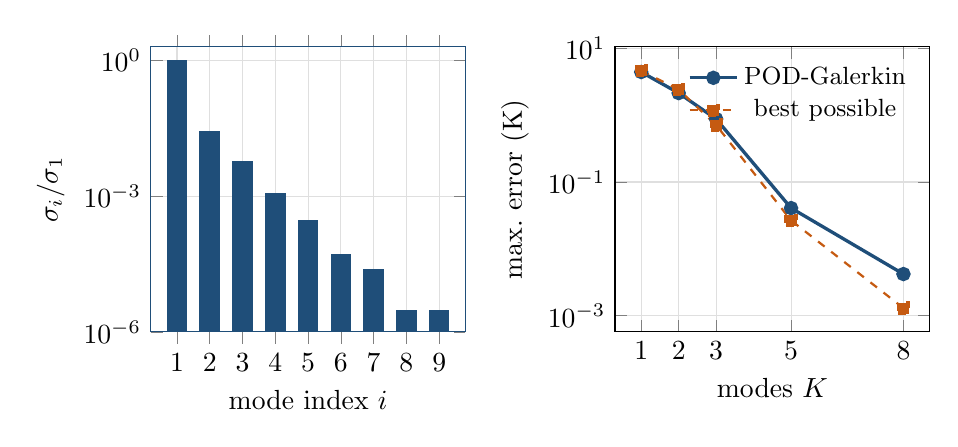
\begin{tikzpicture}
\begin{groupplot}[group style={group size=2 by 1,horizontal sep=1.9cm},width=0.46\linewidth,height=5.2cm,
  grid=major,grid style={gray!25},ymode=log]
\nextgroupplot[ybar,bar width=7pt,log origin=infty,xlabel={mode index $i$},ylabel={$\sigma_i/\sigma_1$},xtick={1,...,9},ymin=1e-6,
  ymax=2,fill=cBlue,draw=cBlue]
  \addplot[fill=cBlue,draw=cBlue] coordinates {(1,1) (2,2.6829e-2) (3,5.954e-3) (4,1.164e-3) (5,2.92e-4) (6,5.1e-5)
     (7,2.4e-5) (8,3e-6) (9,3e-6)};
\nextgroupplot[xlabel={modes $K$},ylabel={max.\ error (\si{\kelvin})},xtick={1,2,3,5,8},
  legend style={font=\small,draw=none,fill=none,at={(0.97,0.97)},anchor=north east}]
  \addplot[cBlue,very thick,mark=*] coordinates {(1,4.3986) (2,2.1301) (3,0.8730) (5,0.0407) (8,0.0042)};
  \addlegendentry{POD-Galerkin}
  \addplot[cOrange,thick,dashed,mark=square*] coordinates {(1,4.6083) (2,2.3997) (3,0.7093) (5,0.0266) (8,0.0013)};
  \addlegendentry{best possible}
\end{groupplot}
\end{tikzpicture}
\caption{Worked example 2. Left: the singular values fall by more than four decades within the first six modes --
two sources and one cooling path need only a few spatial patterns. Right: the Galerkin error falls from
\SI{4.4}{\kelvin} with one mode to \SI{0.04}{\kelvin} (\SI{0.08}{\percent} of the rise) with five modes and stays
within a factor of about 3 of the best error the basis allows. The full model has 1271 states, the reduced model 5:
a reduction by a factor of 250 at an error far below the accuracy of the material data.}
\label{fig:pod}
\end{figure}

\textbf{Interpretation.} The energy criterion alone is misleading here: \SI{99.92}{\percent} energy with one mode
still leaves a \SI{4.4}{\kelvin} error at the hot spot, because the energy is dominated by the large mean heating
pattern and the hot spot is a small region. Choose $K$ from the error at the temperatures that matter (junctions),
not from $E_K$ alone; $E_K\ge 1-10^{-6}$ was needed here for an error below \SI{0.1}{\kelvin}. The column ``without
$h_v$'' shows why the projection must contain every heat sink.

\begin{cfgbox}
\cfg{Mdl › pod › K}: modes $K$ (\cfg{sel = 1}). \cfg{Mdl › pod › sel}: 1 fixed $K$, 2 energy criterion
\cfg{Mdl › gen › Emax} with $K\le$ \cfg{Kmax}. \cfg{Mdl › pod › protocol}: \cref{tab:protocols}.
GUI: \emph{Theory \& Tools › Numerics} explains the quadrature weights and the calibration.
\end{cfgbox}

%######################################################################################################################
\section{POD state space (PS mode)}\label{sec:ps}
%######################################################################################################################
The PS mode keeps the POD modes but \emph{identifies} the dynamics of the modal coordinates instead of projecting the
heat equation:
\begin{equation}
  \bm a(n) = \bm\Phi\T\bigl(\bm T(n)-\bm T_0\bigr),\qquad q_i(n)=\int_\Omega Q(n)\,\phi_i\,\mathrm d\Omega,
\end{equation}
\begin{equation}
  \bm x(n+1) = \mat A\,\bm x(n) + \mat B_d\,\bm q(n),\qquad \bm a(n) = \mat C_o\,\bm x(n),\qquad
  \bm T(n) = \bm T_0 + \bm\Phi\,\mat C_o\,\bm x(n),
\end{equation}
with $K$ modes and $K_s$ states, identified as in \cref{sec:ss} (subspace + output-error fit; every profile is preceded
by $2K_s$ zero samples for a zero initial state). The implementation is dimension independent (2D and 3D).

\begin{keybox}[PO or PS?]
PS needs no material data and no boundary conditions -- only snapshots and losses -- and absorbs model errors of the
data (unknown cooling, FE mesh effects). It only knows the dynamics that the training loads excited and has no
physical structure that guarantees stability or passivity. PO with protocol 2 extrapolates most safely when the
physics in the data is complete; PO with protocol 5 is a compromise. The slowest time constants of both should agree:
they are set by the heat capacity and the cooling.
\end{keybox}

\begin{cfgbox}
\cfg{Mdl › pod › K}, \cfg{sel}, \cfg{Emax} as in the PO mode; \cfg{Mdl › ss › K}: states $K_s$;
\cfg{Mdl › ss › dis/init/sta} as in the SS mode. Start with $K_s\approx K$ to $2K$.
\end{cfgbox}

%######################################################################################################################
\section{Reduced models of the board designer}\label{sec:board}
%######################################################################################################################
The board designer (GUI, \emph{Theory \& Tools}) builds a layer-resolved FV model of a board with chips, thermal vias
and layers below (TIM, heat sink) and reduces it in two ways.

\subsection{POD-Galerkin on the FV grid}
The snapshots of a training run give $\bm\Phi$; the FV matrices are projected directly (\texttt{romBoard}):
$\mat C_r=\bm\Phi\T\mathrm{diag}(\mat C)\bm\Phi$, $\mat G_r=\bm\Phi\T\mat G\bm\Phi$, $\mat B_r=\bm\Phi\T\mat B$. The
reduced model is integrated with the same implicit Euler scheme as the full model, so the difference is the
projection error only (worked example 2).

\subsection{Coupled Cauer network from step responses}
The \emph{thermal characterisation} computes the response of every junction to a \SI{1}{\watt} step in every chip,
$Z_{\mathrm{th},ij}(t)$, on logarithmically spaced times up to the slowest time constant, and the steady-state matrix
$\Rth$. A coupled Cauer network (\cref{sec:sf}) with $K$ stages per chip is fitted to these step responses; its matrices
$\mat G_{\mathrm{th}}$, $\mat C_{\mathrm{th}}$, $\mat E$ can be exported and used e.g.\ as the physics of a PINN
(\cref{sec:pinn}). The junction temperature is either the die average (linear in the losses, superposition is exact,
consistent with data sheets) or the hottest cell of the die (not linear: the maximum of a sum is not the sum of the
maxima, superposition over-estimates it when several chips heat).

\subsection{Electro-thermal coupling}
Losses rise with temperature. Both reduced models can include the linear coupling
$P_{i,\mathrm{eff}} = P_i\max\bigl(1+\alpha_i(T_{j,i}-\Tref),0\bigr)$. The steady state solves
$(\mat G-\mat U\mat W\T)\bm\theta = \mat B\bm P(1+\bm\alpha(T_a-\Tref))$ with $\mat U=\mat B\,\mathrm{diag}(\bm\alpha\bm P)$
(Woodbury identity); a loop gain $\ge1$ means thermal runaway.

%######################################################################################################################
\section{Data-driven models (ML and DL modes)}\label{sec:data}
%######################################################################################################################
When no geometry is available -- e.g.\ an electric motor with only a few temperature sensors and operating data
(currents, voltages, speed, coolant temperature, as in the motor data set of the ML/DL tutorials
\cite{kirchgaessner}) -- the input--output map is learned from profiles.

\subsection{Static regression with smoothed features (ML mode)}
The ML mode fits a static regression $\hat T(n)=f(\bm X(n))$ from the features of one sample to the temperature of the
first node: (1) linear regression, (2) regression tree, (3) support vector regression, (4) Gaussian process
regression, (5) ensemble (boosting or bagging), (6) multilayer perceptron. A static map has no memory; the thermal
memory enters through exponentially weighted moving averages (EWMA) and standard deviations (EWMS) of every feature
(\texttt{calcFeat}):
\begin{equation}
  \mu(n) = \alpha\,x(n) + (1-\alpha)\,\mu(n-1),\qquad
  \sigma^2(n) = (1-\alpha)\bigl(\sigma^2(n-1) + \alpha\,(x(n)-\mu(n-1))^2\bigr),\qquad \alpha=\frac{2}{s+1}.
\end{equation}
The EWMA is a first-order low-pass filter -- the discrete counterpart of one RC pair -- with time constant
$\tau = -T_s/\ln(1-\alpha)\approx sT_s/2$: a span of $s=100$ samples is a \SI{50}{\second} RC pair at $T_s=\SI{1}{\second}$.
A set of spans therefore plays the role of the Foster time constants, and the regression the role of the weights
$R_k$ -- generalised to nonlinear dependencies (e.g.\ losses $\propto I^2$). Choose spans that cover the thermal
time constants of the system.

\subsection{Sequence networks (DL mode)}
The DL mode maps a window of $W$ samples of $F$ features ($W\times F$, z-score normalised) to the temperatures of all
$M$ nodes with a convolutional (CNN), recurrent (LSTM, GRU) or attention (transformer) network or a user-defined layer
list. \emph{seq2point} (\cfg{Mdl › dl › seq} $=s>0$) predicts sample $s$ of the window ($s=W$: causal, only past
inputs); \emph{seq2seq} ($s=0$) predicts every sample of the window. The window must cover the dominant time constant
($WT_s\gtrsim\tau_{\max}$), otherwise the network cannot know the thermal history. Training uses Adam with a
learning-rate schedule, gradient clipping and early stopping on the validation loss; the network with the lowest
validation loss is kept.

\begin{keybox}[Strengths and limits]
Data-driven models capture nonlinearities (temperature-dependent losses, speed-dependent cooling) that linear
reduced models cannot. They need much data covering the whole operating range, they give no physical parameters, and
they can fail silently outside the training range. Always test on profiles that were not used for training or
validation.
\end{keybox}

\begin{cfgbox}
ML: setup \cfg{selML} (1--6), \cfg{featRoll}, \cfg{EWMA}, \cfg{EWMS}; \cfg{Mdl › gen › opt = 1} random search of the
hyperparameters (3-fold cross validation). DL: setup \cfg{selDL} or \cfg{archDL}; \cfg{Mdl › dl › W, seq, stride,
epoch, batch, initLr, lrAdapt, lrDropPr, lrDropFa, gradTh, valFreq, valPat, loss}; \cfg{Mdl › gen › dev = 1} GPU.
\end{cfgbox}

%######################################################################################################################
\section{Physics-informed neural network (PI mode)}\label{sec:pinn}
%######################################################################################################################
The PINN \cite{raissi} combines a sequence network with a lumped thermal network. The network predicts the states $\bm x$ of the
physics model
\begin{equation}
  \mat C\,\dot{\bm x} = \mat E\,\bm P(t) - \mat G\,\bm x,\qquad \hat T_i = T_{\mathrm{ref},i} + (\mat O\bm x)_i ,
\end{equation}
where the physics is (0) none, (1) Foster chains between sources and outputs (one state per term,
$\tau_k\dot\theta_k = R_kP_j-\theta_k$) or (2) a Cauer/nodal network with hidden nodes (e.g.\ from the SF mode or the
board designer). The losses $P_j$ are equations of the input features (e.g.\ $3R_sI^2$ for copper losses). Training
minimises three dimensionless parts ($\Delta T$: temperature scale of the training data):
\begin{equation}
  L = \alpha\,\underbrace{\mathrm{mean}\Bigl(\tfrac{\hat T - T}{\Delta T}\Bigr)^2}_{L_{\mathrm{data}}}
    + \beta\,\underbrace{\mathrm{mean}\Bigl(\tfrac{\mat C\dot{\bm x}+\mat G\bm x-\mat E\bm P}{\mathrm{diag}(\mat G)\,\Delta
      T}\Bigr)^2}_{L_{\mathrm{phys}}}
    + \gamma\,\underbrace{\frac{\sum w\,\bigl(\tfrac{\hat T-T(0)}{\Delta T}\bigr)^2}{\sum w}}_{L_{\mathrm{init}}},
    \quad w=e^{-t/\tau_{\min}} .
\end{equation}
$L_{\mathrm{data}}$ is evaluated where temperatures are measured, $L_{\mathrm{phys}}$ for every state and also on
\emph{collocation profiles} (inputs without measured temperatures, \cfg{Mdl › pinn › col}), $L_{\mathrm{init}}$ keeps
the prediction at the measured start temperature. The first \cfg{warm} samples of every window are excluded (the
recurrent state settles).

\begin{keybox}[When the physics helps]
The physics loss acts as a regulariser: with little labelled data and an accurate physics model it constrains the
network where no temperatures are measured (example in the GUI theory view: one labelled profile, test RMSE
\SI{12}{\kelvin} $\to$ \SI{4}{\kelvin} with six unlabelled profiles). If the physics is simplified, a large $\beta$
makes the network follow the wrong physics; $\beta=0.01$--$1$ is the useful range.
\end{keybox}

\begin{cfgbox}
\cfg{Mdl › pinn › phys} (0/1/2), \cfg{alpha}, \cfg{beta}, \cfg{gamma}, \cfg{warm}, \cfg{pred}, \cfg{x0}, \cfg{col},
\cfg{TrefSrc}, \cfg{Tref}, \cfg{node}; setup \cfg{selPI} or \cfg{archPI}, \cfg{physPI} (GUI view \emph{Physics}).
\end{cfgbox}

%######################################################################################################################
\section{Comparison and selection guide}\label{sec:select}
%######################################################################################################################
\begin{table}[h]\centering\footnotesize
\caption{Properties of the reduced model families. ``Extrapolation'' rates how safely the model predicts loads that
differ from the training loads (+++: physics-based, ++: linear identified, +: learned).}\label{tab:compare}
\setlength{\tabcolsep}{3.5pt}
\begin{tabularx}{\linewidth}{@{}l>{\raggedright\arraybackslash}X>{\raggedright\arraybackslash}p{1.9cm}>{\raggedright\arraybackslash}p{2.5cm}cc>{\raggedright\arraybackslash}X@{}}\toprule
Mode & Needs & Returns & Parameters & Coupl. & Extrap. & Typical use \\\midrule
RC & 1 loss, 1 temperature & 1 temperature & $2K$ & no & ++ & data-sheet $\Zth$, single chip, lifetime \\
SS & all losses and temperatures & $p$ temperatures & $n_x^2+n_x(m+p)$ & yes & ++ & MIMO, observers, control \\
SF & profiles of $M$ chips & $M$ junctions & $\approx M(2K)+KM(M-1)/2$ & yes & ++ & power modules, inverter legs \\
PO & FE snapshots + material data & full field & $\approx 2K^2+K$ & yes & +++ (prot.\ 2) & hot spots, sensor placement \\
PS & FE snapshots + losses & full field & $K_s^2+2K_sK$ + modes & yes & ++ & field without material data \\
ML & operating data & 1 temperature & model-dependent & -- & + & motors, quick static estimates \\
DL & much operating data & $M$ temperatures & $10^4$--$10^5$ & -- & + & nonlinear systems, rich data \\
PI & data + lumped physics & $M$ temperatures & $10^4$--$10^5$ & yes & + to ++ & little data, known structure \\\bottomrule
\end{tabularx}
\end{table}

\begin{figure}[h]\centering
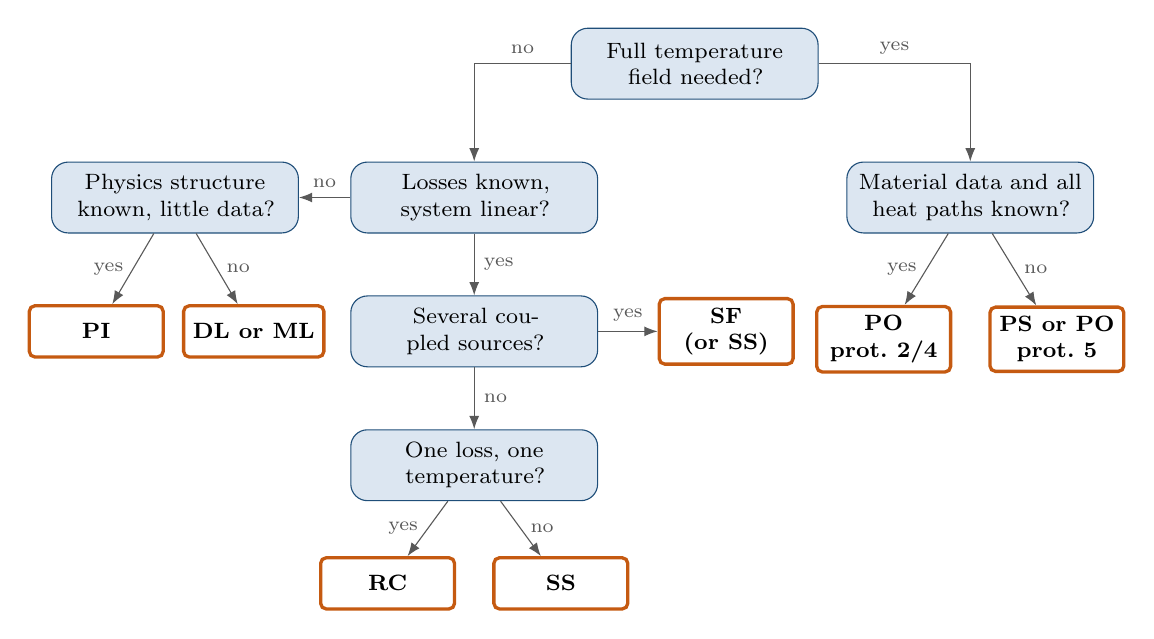
\begin{tikzpicture}[
  q/.style={draw=cBlue,fill=cLight,rounded corners=6pt,align=center,font=\footnotesize,text width=2.9cm,
            minimum height=0.9cm},
  a/.style={draw=cOrange,very thick,fill=white,rounded corners=2pt,align=center,font=\footnotesize\bfseries,
            minimum width=1.7cm,minimum height=0.65cm},
  arr/.style={-{Latex},cGrey},lab/.style={font=\scriptsize,text=cGrey}]
  \node[q] (q1) at (1.6,0) {Full temperature field needed?};
  \node[q] (q2) at (5.1,-1.7) {Material data and all heat paths known?};
  \node[a] (po) at (4.0,-3.5) {PO\\prot.\ 2/4};
  \node[a] (ps) at (6.2,-3.5) {PS or PO\\prot.\ 5};
  \node[q] (q3) at (-1.2,-1.7) {Losses known, system linear?};
  \node[q] (q6) at (-5.0,-1.7) {Physics structure known, little data?};
  \node[a] (pi) at (-6.0,-3.4) {PI};
  \node[a] (dl) at (-4.0,-3.4) {DL or ML};
  \node[q] (q4) at (-1.2,-3.4) {Several coupled sources?};
  \node[a] (sf) at (2.0,-3.4) {SF\\(or SS)};
  \node[q] (q5) at (-1.2,-5.1) {One loss, one temperature?};
  \node[a] (rc) at (-2.3,-6.6) {RC};
  \node[a] (ss) at (-0.1,-6.6) {SS};
  \draw[arr] (q1.east) -| node[lab,above,pos=0.25]{yes} (q2.north);
  \draw[arr] (q1.west) -| node[lab,above,pos=0.25]{no} (q3.north);
  \draw[arr] (q2) -- node[lab,left]{yes} (po);
  \draw[arr] (q2) -- node[lab,right]{no} (ps);
  \draw[arr] (q3) -- node[lab,above]{no} (q6);
  \draw[arr] (q6) -- node[lab,left]{yes} (pi);
  \draw[arr] (q6) -- node[lab,right]{no} (dl);
  \draw[arr] (q3) -- node[lab,right]{yes} (q4);
  \draw[arr] (q4) -- node[lab,above]{yes} (sf);
  \draw[arr] (q4) -- node[lab,right]{no} (q5);
  \draw[arr] (q5) -- node[lab,left]{yes} (rc);
  \draw[arr] (q5) -- node[lab,right]{no} (ss);
\end{tikzpicture}
\caption{Selection guide. ``Linear'' means that the losses are known inputs and the material properties hardly
depend on temperature; temperature-dependent losses can still be handled by the electro-thermal coupling of the
board designer or by the loss equations of the PINN.}
\label{fig:select}
\end{figure}

\textbf{Practical recommendations.}
\begin{itemize}
  \item Start simple: an RC or SS model on the same data gives a baseline for every more complex model.
  \item Sample at least 3--5 times faster than the fastest time constant you need; record at least 3--5 times the
        slowest one.
  \item Excite every source on its own at least once (single-source steps or random levels with independent
        amplitudes): otherwise cross-heating cannot be separated from self-heating (\cref{sec:sf}).
  \item Choose the order from the validation error at the temperatures that matter, not from the training error or the
        POD energy alone.
  \item Test on a profile that differs from the training profiles (different frequency content and amplitudes).
\end{itemize}

\subsection*{Other MOR methods (not implemented)}
For completeness: \emph{balanced truncation} keeps the states that are both well controllable and well observable
(Hankel singular values) and has an a-priori error bound \cite{antoulas}; \emph{Krylov / moment matching} methods
(PRIMA, Arnoldi) match the low-frequency behaviour of large FE models and keep passivity \cite{antoulas}. Both need the
system matrices of the full model; TherMOS works from data (snapshots, profiles), which is why it uses POD and system
identification.

%######################################################################################################################
\section{Error metrics}\label{sec:metrics}
%######################################################################################################################
All modes report the same metrics per output channel (\texttt{calcError}) with $e=y-\hat y$ over $N$ samples:
\begin{table}[h]\centering\small
\begin{tabularx}{\linewidth}{@{}lllX@{}}\toprule
Metric & Definition & Unit & Meaning \\\midrule
MAE & $\frac1N\sum|e|$ & \si{\kelvin} & mean absolute error; typical deviation \\
RMSE & $\sqrt{\frac1N\sum e^2}$ & \si{\kelvin} & root mean square error; weights large errors more \\
MAX & $\max|e|$ & \si{\kelvin} & largest deviation; relevant for temperature limits \\
SAE & $(\overline{|y|}-\overline{|\hat y|})/\overline{|y|}$ & p.u. & relative error of the mean level (sign: bias) \\
NAE & $\sum|e|/\sum|y|$ & p.u. & absolute error relative to the signal \\
FIT & $100\,(1-\lVert e\rVert/\lVert y-\bar y\rVert)$ & \si{\percent} & fit percentage as MATLAB \texttt{compare}; 100 = perfect, 0 = as good as the mean \\
NRMSE & $100\,\mathrm{RMSE}/(\max y-\min y)$ & \si{\percent} & RMSE relative to the temperature swing \\\bottomrule
\end{tabularx}
\end{table}

For temperatures in \si{\celsius} the relative metrics SAE and NAE depend on the offset of the scale; compare models
with MAE, RMSE, MAX and NRMSE.

%######################################################################################################################
% References
%######################################################################################################################
\begin{thebibliography}{9}
\bibitem{antoulas} A.\ C.\ Antoulas, \emph{Approximation of Large-Scale Dynamical Systems}. SIAM, 2005.
\bibitem{holmes} P.\ Holmes, J.\ L.\ Lumley, G.\ Berkooz, C.\ W.\ Rowley, \emph{Turbulence, Coherent Structures,
  Dynamical Systems and Symmetry}, 2nd ed. Cambridge University Press, 2012.
\bibitem{verhaegen} M.\ Verhaegen, V.\ Verdult, \emph{Filtering and System Identification: A Least Squares
  Approach}. Cambridge University Press, 2007.
\bibitem{vanoverschee} P.\ Van Overschee, B.\ De Moor, \emph{Subspace Identification for Linear Systems}. Kluwer, 1996.
\bibitem{ljung} L.\ Ljung, \emph{System Identification: Theory for the User}, 2nd ed. Prentice Hall, 1999.
\bibitem{jesd51} JEDEC, \emph{JESD51-14: Transient Dual Interface Test Method for the Measurement of the Thermal
  Resistance Junction-to-Case of Semiconductor Devices with Heat Flow Through a Single Path}, 2010.
\bibitem{raissi} M.\ Raissi, P.\ Perdikaris, G.\ E.\ Karniadakis, ``Physics-informed neural networks,''
  \emph{J.\ Comput.\ Phys.}, vol.\ 378, pp.\ 686--707, 2019.
\bibitem{kirchgaessner} W.\ Kirchgässner, O.\ Wallscheid, J.\ Böcker, ``Electric Motor Temperature'' data set, Kaggle,
  CC BY-SA 4.0.
\bibitem{thermos} P.\ A.\ Schirmer, ``TherMOS: A Robust Low-Resolution 2D Spatial Thermal Model Order Reduction
  Approach'' (setup files in \texttt{setup/journal}).
\end{thebibliography}

\end{document}
